\subsection{Interrelación Alumno Curso Académico - Alumno}

   \begin{description}
      \item[Definición] En esta interrelación se deja constancia de que un
      alumno puede estar matriculado durante un número indeterminado de cursos
      académicos.

      \item[Características] La interrelación presenta las siguientes
                             características:

         \begin{itemize}
            \item \textbf{Nombre:} AlCA-A
            \item \textbf{Tipo de la interrelación:} El tipo de entidad
                  Alumno Curso Académico es débil por identificación respecto al
                  tipo de entidad Alumno.
            \item \textbf{Cardinalidad de la interrelación:} N:1
            \item \textbf{Número de atributos:} Ninguno.
         \end{itemize}

      \item[Diagrama] La figura \ref{diagramaAlCA-A} muestra el diagrama de la
                      interrelación.

      \item \begin{figure}[!ht]
            \begin{center}
            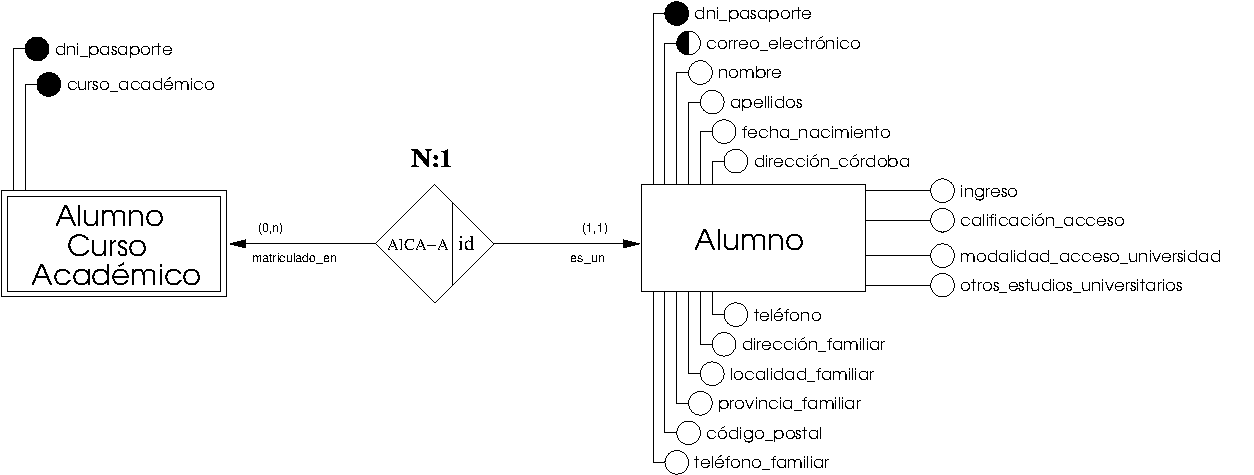
\includegraphics[]{07.Modelo_Entidad-Interrelacion/7.3.Analisis_Interrelaciones/diagramas/AlCA-A.pdf}
            \caption{Diagrama de la interrelación AlCA-A.}
            \label{diagramaAlCA-A}
            \end{center}
         \end{figure}

      \item[Ejemplo práctico del tipo de interrelación]

      \item \begin{center}
            \begin{tabular}{ | c | c | }
            \hline
            \multicolumn{2}{ | c | }{\textbf{Tipo de interrelación AlCA-A}} \\
            \hline
            \textbf{Alumno Curso Académico} & \textbf{Alumno}\\
            \hline
            dni\_pasaporte+id\_centro & dni\_pasaporte \\
            \hline
            01234567A2008 & 01234567A \\
            \hline
            \end{tabular}
         \end{center}
   \end{description}
